


\chapter{Экспериментальная часть}\label{exp}
%\addcontentsline{toc}{chapter}{4 Экспериментальная часть}

Оценка качества работы алгоритмов. Экспериментальное сравнение работы различных алгоритмов умножения матриц 
(зависимость времени выполнения от размерности матриц).

\section{Примеры работы}\label{examples}

На рисунках \ref{ris:w1}, \ref{ris:w2}, \ref{ris:w3}, \ref{ris:w4}, \ref{ris:w5} показаны примеры работы.

\begin{figure}[H]
    \center{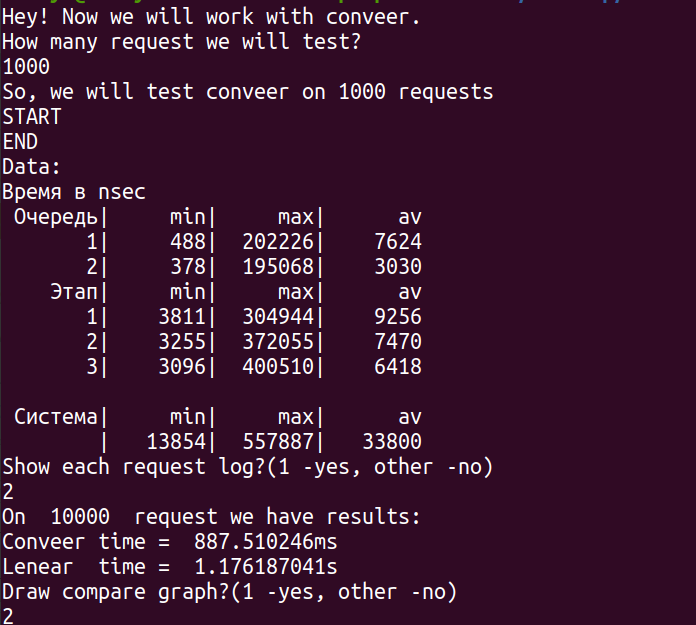
\includegraphics[scale=0.35]{w1}}
    \caption{Ручное тестирование: тест 1}
    \label{ris:w1}
\end{figure}
  
\begin{figure}[H]
    \center{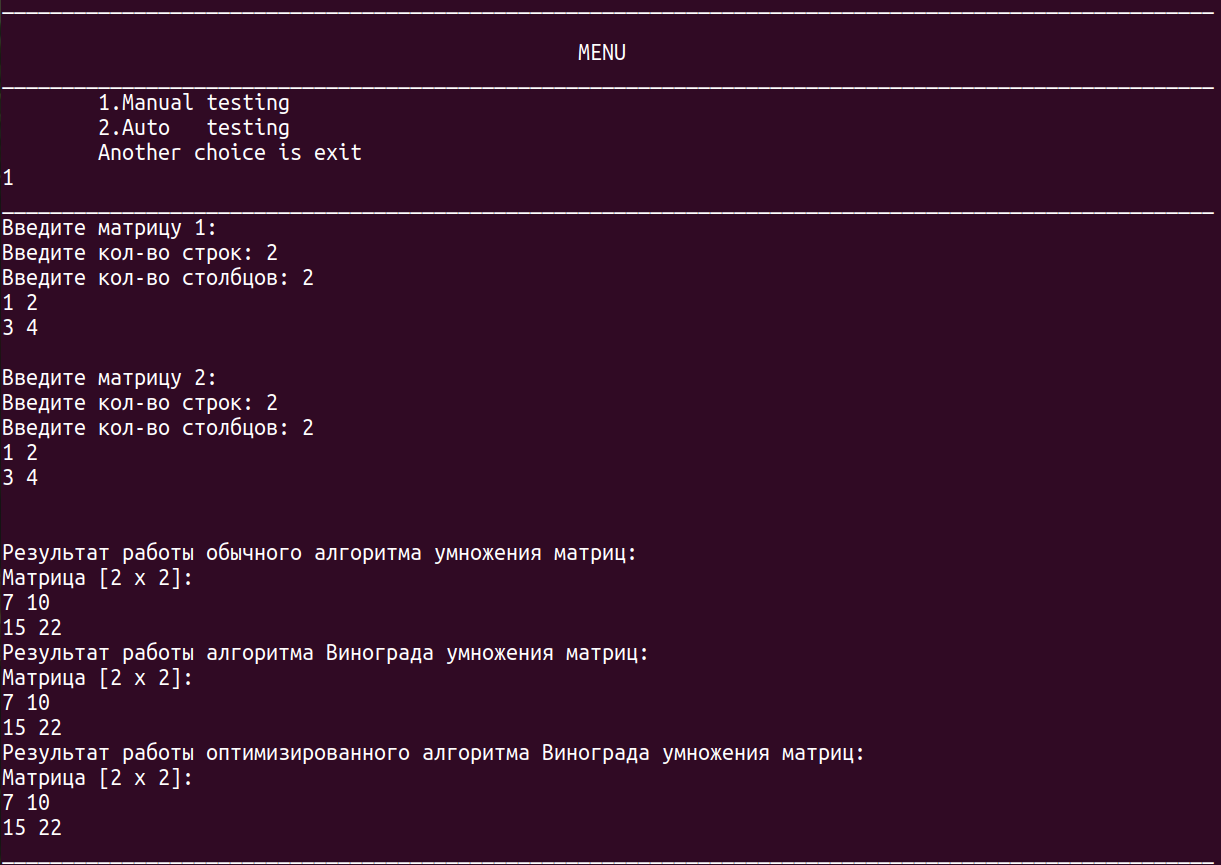
\includegraphics[scale=0.35]{w2}}
    \caption{Ручное тестирование: тест 2}
    \label{ris:w2}
\end{figure}
  
\begin{figure}[H]
    \center{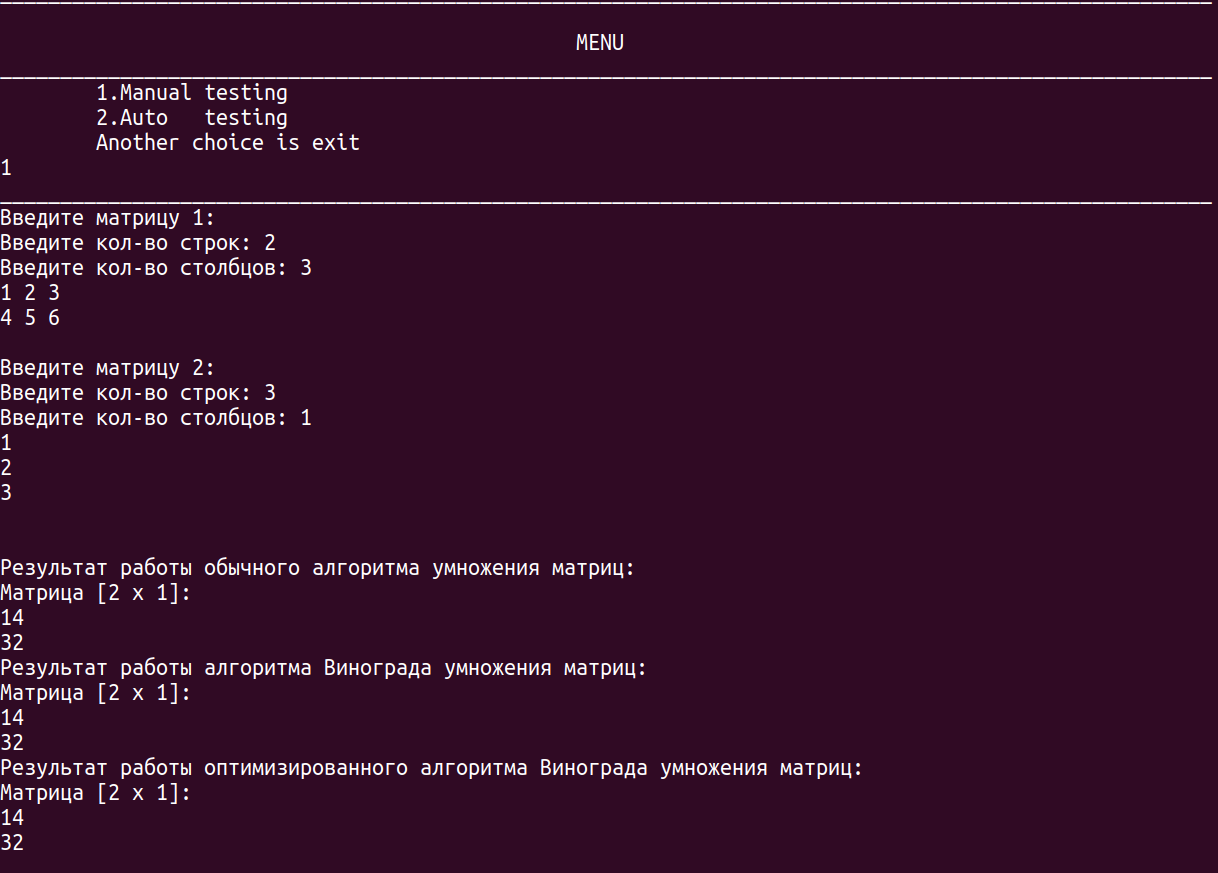
\includegraphics[scale=0.35]{w3}}
    \caption{Ручное тестирование: тест 3}
    \label{ris:w3}
\end{figure}
  
\begin{figure}[H]
    \center{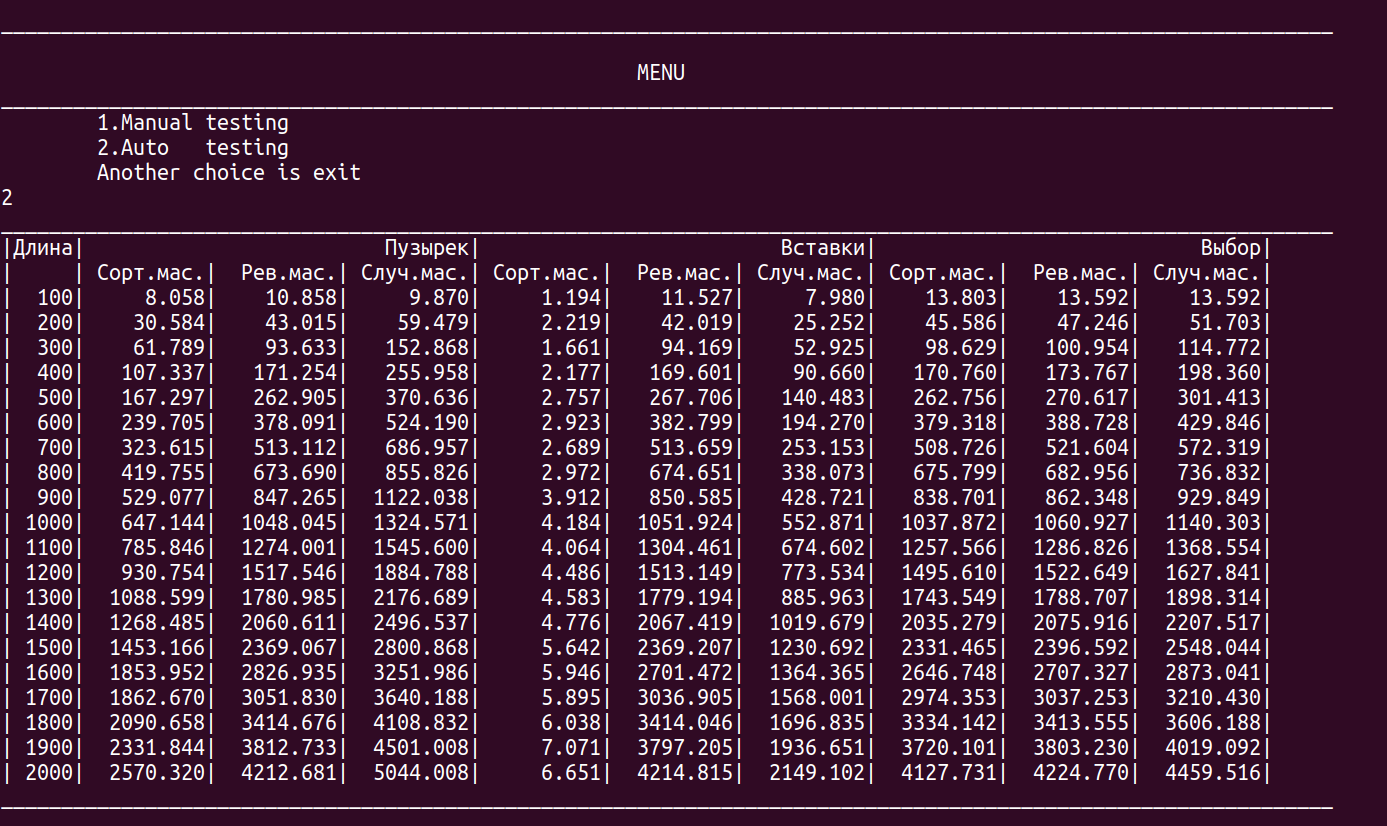
\includegraphics[scale=0.25]{w4}}
    \caption{Автотестирование}
    \label{ris:w4}
\end{figure}
\section{Замеры времени}\label{experimentgraph}

На рисунках \ref{ris:graph1}, \ref{ris:graph2}, и \ref{ris:graph3} показаны графические результаты сравнения исследуемых алгоритмов по времени. 

\begin{figure}[H]
    \center{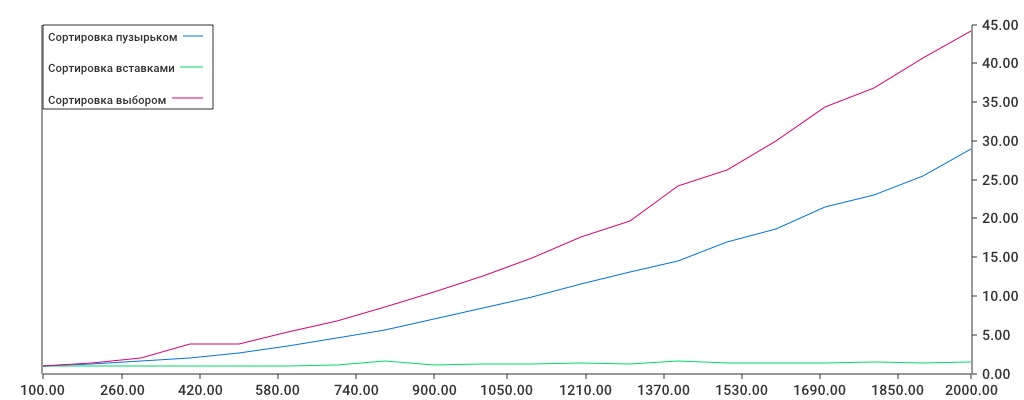
\includegraphics[scale=0.4]{../Lab3/output.png}}
    \caption{Сравнение 3 исследуемых алгоритмов по времени (массив отсортирован)}
    \label{ris:graph1}
\end{figure}

\begin{figure}[H]
    \center{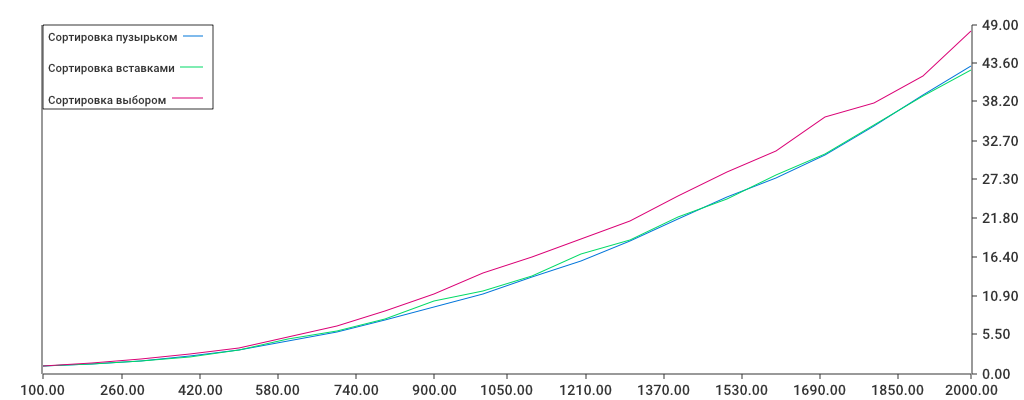
\includegraphics[scale=0.4]{../Lab3/output2.png}}
    \caption{Сравнение 3 исследуемых алгоритмов по времени (массив отсортирован в обратном порядке)}
    \label{ris:graph2}
\end{figure}

\begin{figure}[H]
    \center{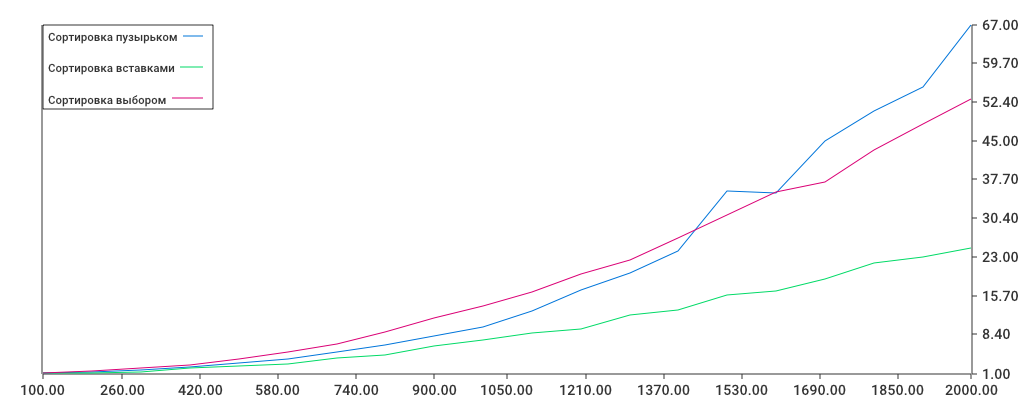
\includegraphics[scale=0.4]{../Lab3/output3.png}}
    \caption{Сравнение 3 исследуемых алгоритмов по времени (массив сгенерирован случайно}
    \label{ris:graph3}
\end{figure}

\section{Сравнительный анализ алгоритмов}\label{comparepart}

Были протестированы алгоритмы сортировки. Самый эффективный из исследуемых алгоритмов по времени на отсортированном массиве - сортировка 
вставками, самый медленный - сортировка пузырьком. На отсортированном в обратном порядке массиве сортировки вставками и пузырьком 
приблизительно одинаковы по скорости и они быстрее сортировки выбором, то есть самый медленный алгоритм - сортировка пузырьком. Самый 
эффективный из исследуемых алгоритмов по времени на случайном массиве - сортировка вставками, при длине массива меньше 1400 сортировка 
пузырьком быстрее сортировки выбором, при большем количестве эллементов сортировка пузырьком медленее сортировки выбором. 


\section{Вывод экспериментальной части}\label{experimentresult}

Таким образом, подтвердилось предположение, что самый эффективный алгоритм в лучшем случае алгоритм - сортировка вставками, а самый 
медленный сортировка пузырьком. Предположение о худшем случае оказалось неверно. Быстрыми алгоритмами в этом случае являются сортировки 
вставками и пузырьком, самый медленный - сортировка выбором.

\chapter{Заключение}\label{exit}

В данной работе были изучены алгоритмы сортировки массива: пузырьком, выбором, вставками. 
Получены практические навыки реализации исследуемых алгоритмов. Была подсчитана трудоемкость исследуемых алгоритмов. 
Проведён сравнительный анализ алгоритмов по времени и трудоемкости. 
Экспериментально подтверждены различия в эффективности алгоритмов с указанием лучших и худших случаев. 
Цель работы достигнута, решены поставленные задачи. 
Получены практические навыки реализации алгоритмов сортировки, а также проведена исследовательская работа 
вычислении трудоемкости алгоритмов.
